\subsection{Descripción del problema.}

\vspace*{0.3cm}



\textbf{Introduccion al problema} \newline

Como es sabido en la Republica Argentina y talvez otros paises, las sistema ferreo esta distribuido en forma de abanico como en la \textbf{figura 1}.
En el ejemplo de abajo tenemos todas las lineas ferroviarias, tienen como origen la Capital Federal.
\begin{figure}[htb]
	\begin{center}
		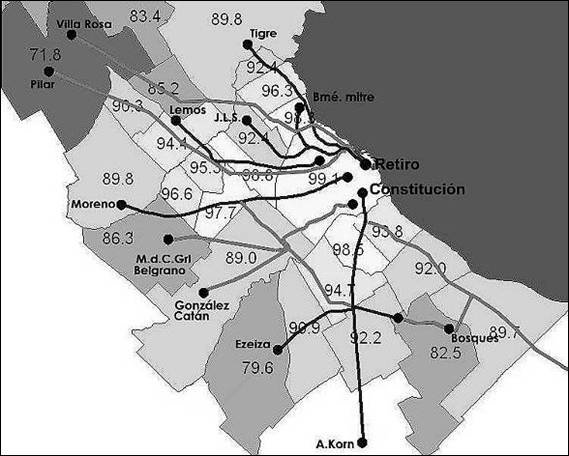
\includegraphics[scale=0.50]{imagenes/red-trenes.jpg}
	\end{center}
	\caption{Trenes provincia de Buenos Aires, Argentina}
\end{figure}
Y cada linea ferroviarria tiene una estacion inicial y las estaciones que le siguen a la inicial. Como por ejemplo en la \textbf{figura 2}, donde la estacioon inicial Retiro, Saldias, ... , Villa Rosa. 
Cada estacion esta ubicada una cierta distancia respecto de la estacion inicial.
Por ejemplo:

\begin{figure}[htb]
	\begin{center}
		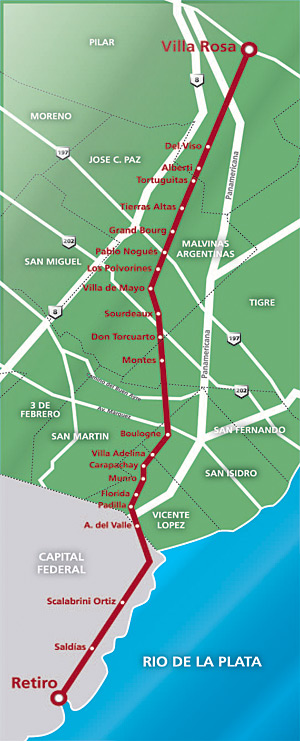
\includegraphics[scale=0.25]{imagenes/Belgrano-Norte.jpg}
	\end{center}
	\caption{Linea de tren Belgrano Norte}
\end{figure}

Cada estacion esta ubicada una cierta distancia respecto de la estacion inicial.
Por ejemplo:
\begin{center}
   \begin{tabular}{ | l | c | r | }
     \hline
     estacion & distancia a estacion Retiro \\ \hline
     Retiro  & 0 \\ \hline
     Saldias  & 5\\ \hline
     Scalabrini Ortiz & 10 \\ \hline
     Aristobulo Del Valle & 14 \\ \hline
     ... & ... \\ \hline
     Villa Rosa & 60 \\ 
     \hline
   \end{tabular}
\end{center}

\textbf{Problema concreto} \newline

Nos han encomendo el trabajo de conectar telegraficamente todas las estaciones del sistema ferreo,
para cada linea del sistema ferreo se le destinara una cantidad en metros de cable y deberemos conectar maxima cantidad posible de estaciones. Dicho cable no debera cortarse, sino que su uso con el cable entero.

Este es un tipico problema de optimizacion en este caso de trata de una maximizacion.
El objetivo nuestro es la busqueda de un algoritmo que pueda conectar la mayor cantidad de estaciones de una linea ferrea con el uso de un solo cable de determinada longitud.  

Nuestro input esta compuesta por la primer linea donde se indica la longitud de cable destinada para esa linea ferrea. La siguiente linea seran una serie 
de numeros separados por un espacio y ordenados de manera no decreciente (osea estrictamente creciente), donde cada numero representa la distancia hacia la $estacion_0$. 
Respecto a la serie de numeros:
\begin{itemize}
    \item La $estacion_0$ no esta en la serie pues su distancia hacia si misma es $0$.
    \item la serie comienza con la distancia de la $estacion_1$, $estacion_2$, ...., $esta4cion_n$, todas las distancia son respecto a la $estacion_0$ 
\end{itemize}

\textbf{Ejemplo input y sus respectivos output: } 

\begin{center}
   \begin{tabular}{ | l | c | r | }
     \hline
     longitud cable(input) & distancias de estaciones(input) & maxima cantidad de ciudades (output)\\ \hline
     4 & 1 4 6 7 8 9 & 4 \\ \hline
     2 & 1 2 3 4 5 6 7 & 3 \\ \hline
     7 & 1 2 3 4 5 6 7 & 8 \\ \hline
     2 & 4 8 15 & 0 \\
     \hline
   \end{tabular}
\end{center}


%	\begin{figure}[htb]
%  \begin{center}
%      \includegraphics[scale=0.25]{imagenes/red-ferroviaria.jpg}
%	  \end{center}
% \caption{ejemplo}
%\end{figure}

\newpage
\subsection{Desarrollo de la idea y pseudocódigo.}

\vspace*{0.3cm}

%\textbf{completar.}
\textbf{}
Para el desarrollo de nuestro algoritmo pusimos todas distancias de las estaciones en un arreglo en el orden en que venian i ademas agregamos la estacion_0 con distancia 0, la longitud del cable fue almacenada en un entero.
 
Nuestro algoritmo utiliza un bucle principal el cual podria iterar $n$ veces, y cada itercion verifica que no nos hayamos pasado de longitud del arreglo.
Para el controlar las la cantidad de iteraciones que hacemos usamos dos variables que vamos a llamar $desde$ y $hasta$, donde estas variables marcar en que subarreglo estamos ubicados. En cada iteracion lo que hacemos es empezar a contar las ciudades desde donde dejamos $desde+1$ y $hasta-1$, esto me asegura que itere solamente n veces. De ahi que vamos a llega deducir que el algoritmo en lineal al tamanio de la entrada. 


\textbf{pseudocodigo} \newline 

\begin{codebox}
\Procname{$\proc{maximasEstacionesConectadas}(array<int> \ estaciones,Nat \ mCables)	$}
	\li inicializamos las variables enteras $desde$,$hasta$,$cantEstacionesConectadas$,$cantidadDeEstacionesMaxima$ en 0.
	\li inicializamos las variables booleana $mePase$ en $false$.
	\li \While $(hasta < estaciones.length -1)$
	\li \Do	 // veo cuantas estaciones pudo unir con el cable.
		\li \While ($hasta<estaciones.length \land estaciones[hasta]-estaciones[desde]<=mCable$) 
		\li \Do	
				\li $hasta++$ // porque agregamos una estacion mas
				\li $mePase \leftarrow true$.
			\End
			\li \If $mePase$ 
			\li \Then 
					$hasta \leftarrow hasta-1;$
					$ mePase \leftarrow False;$
			\End		
			\li $cantEstacionesConectadas$ es Cero si $desde==hasta$ , sino $hasta-desde + 1$
			\li $cantidadDeEstacionesMaxima \leftarrow$ Max( $cantidadDeEstacionesMaxima$,$cantEstacionesConectadas$);
			\li $desde \leftarrow desde+1$  
		\End	
	\End
	\li \Return $\id{cantidadDeEstacionesMaximas}$ // retorno la mayor cantidad de estaciones que se pudieron conectar
	      
\end{codebox}

\newpage
\subsection{Justificación de la resolución y demostración de correctitud.}

\vspace*{0.3cm}

\textbf{Teorema: } El algoritmo golozo utilizado encuentra siempre una solucion optima (donde solucion optima se refiere a conectar la mayor cantidad de estaciones posible).

\textbf{Demostracion: } Probaremos que dada una solucion optima $S$, el algoritmo genera una solucion $S'$ con por lo menos la misma cantidad de estaciones que la solucion $S$, es decir que la solucion generada por el algoritmo golozo es optima. \newline
Supongamos por el \underline{absurdo} que la solucion $S'$ dada por el algoritmo golozo no es optima y tomaremos la solucion optima $S$ que mas estaciones comparta con con la solucion brindada por el algoritmo golozo $S'$.
\newline
por ejemplo: $estaciones = \{x_1 x_2 x_3 x_4 x_5 x_6 x_7 \}$ ,  $S =\{ x_2 x_3 x_4 x_5 x_6\}$  y  $S'=\{ x_2 x_3 x_4 x_5\}$.  
\newline
Sean $S$ el secuencia de solucion optima y $S'$ la secuencia brindada por el algoritmo golozo.
Supongamos ademas que ambas secuencas tienen el mismo origen (osea, $S_1$ == $S'_1$).
Sea $S_j$ el primer elemento distinto del los elementos de $S'$ ($S_j$ existe pues supusimos que $S'$ no optimo), en pocas palabras 
para todo $i<j$ vale $S_i = S'_j$. De esta manera sabemos que podemos conectar $S_{j-1}$ con $S_{j}$ pues es solucion optima.
Pero entonces $S'_j$ es elegido por nuestro algoritmo como elemento que se conecta con $S'_{j-1}$, entonces debe suceder que $S_j = S'_j$.
Pero llegamos a que $S = S'$ comparten todos los puntos entonces llegamos a que $S'$ es optimo absurdo.\newline
El absurdo viene de supóner que $S'$ no es optimo.   	



%\newpage
\subsection{Análisis de complejidad propuesta.}
La complejidad de mi algoritmo es $O(n)$, pero al tener dos ciclos anidados. No esta demas decir que  en ambos ciclos realizamos operaciones que cuestan $O(1)$,  ya que son operaciones aritmeticas(sumas, restas), asignaciones.
Como se desprende del pseudocodigo que como mucho el ciclo mayor(linea 3 pseudocodigo)va ciclar n veces y como poco cicla 1 ves.
 Veamos algunos casos:  
 \begin{itemize}
    \item Caso en el que el ciclo mayor cicla 1 vez, dentro del ciclo mayor tenemos un ciclo menor(linea 5 pseudocodigo) que ciclara la $n-1$ veces que me faltan ciclar y con esto ya tendiramos las n iterciones. Ejemplo de esto seria por ejemplo que el cable pudiera conectar a todas las estaciones ($estaciones=\{1,2,3,4,5,6\})y$ $mCable= 6$).
    \item El caso en que el ciclo mayor cicla n veces pordria ser por ejemplo que no podamos conectar niguna ciudad, por lo tanto el ciclo menor costaria $O(1)$ y el ciclo mayor ciclaria $n$ veces. Ejemplo: $estaciones = \{4,8,12\}, mCable = 3$, como vemos no podemos conectar ninguna estacion,
    \item Hay casos intermedios que son de  similar analisis.
\end{itemize}

Podemos deducir que la complejidad de el algoritmo es $O(n)$, ya que los dos ciclos estan interrelacionados, la variable ''hasta'' solo puede llegar a n. Para el ciclo anidado mas externo en cada iteración, incrementa la variable ''hasta'' una cierta cantidad de veces, finalmente incrementa la variable ''desde''. Aunque solo se incremente una o cero veces la variable ''hasta'', lo estará haciendo la variable ''desde'', y como siempre ''desde'' $ \leq $ ''hasta'', tenemos a lo sumo n incrementos para la variable ''desde'' y n para ''hasta''.
 

\subsection{Experimentación y gráfico.}

\vspace*{0.3cm}
En las secciones anteriores nos ocupamos de la complejidad teorica.
Ahora lo que nos interesara  es contrastar lo teorico con lo experimental, lo haremos haciendo experimento, los cuales plasmaremos en un grafico. 
Como ya habiamos comentado en la parte de analisis de complejidad, nuestro algoritmo teoricamente no tiene un peor y mejor. Por consiguiente(caso peor, mejor, aleatorio) los graficos seran todos similares entre si.   

\begin{figure}[htb]
  \begin{center}
      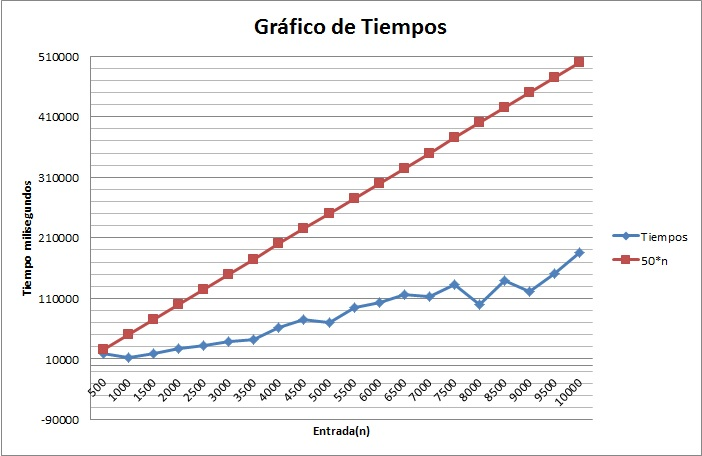
\includegraphics[scale=0.75]{imagenes/GraficoEj1.jpg}
  \end{center}
  \caption{ejemplo}
\end{figure}


Para tomar los tiempos utilizamos instancias de tamaños entre 500 a 10000 elementos. 
Lo que hicimos fue para cada instancia correr 200 veces el algoritmo golozo y tamamos el promedio de los resultados que tuvieran una variación estándar.
Para hacer esto filtramos los tiempos y nos quedamos con aquellos que estubieran entre el promedio menos el desvío estándar y promedio mas el desvío estándar.El desvío estándar mide cuanto tienden a alejarse los resultados del promedio. Para calcular el desvío, primero tuvimos que calcular la varianza. Para obtener la varianza agarramos cada uno de los tiempos y  les restamos el promedio y lo elevamos al cuadrado, después tomamos el promedio de esos resultados. Para terminar de calcular el desvío solo sacamos la raíz cuadrada de la varianza. Para hacer esto
\newline
Como podemos apreciar en el gráfico nuestro  algoritmo tiende a tener una complejidad exactamente lineal, ya que a simple vista la podemos acotar superiormente e inferiormente por n. \newline
\textbf{Observación: } utilizamos el desvío estándar porque la computadora puede tardar mucho mas o mucho menos, lo que haces es tomar el promedio de las cosas que no se va muy por fuera de lo esperado
	


%\newpage
%\subsubsection{Test 2}

%\vspace*{0.3cm}

%\textbf{completar!}


%\newpage
%\subsubsection{Test 3}

%\vspace*{0.3cm}

%\textbf{completar!}
